%!TEX encoding = utf8
%!TeX spellcheck = en_GB
%%%%%%%%%%%%%%%%%%%%%%%%%%%%%%%%%%%%%%%%%%%%%%%%%%%%%%%%%%%%%%%%%%
\documentclass[10pt]{thesis}

\usepackage[utf8]{inputenc}
\usepackage[T1]{fontenc}
\usepackage[a4paper, total={7in, 9in}]{geometry} %Din A4

\usepackage{graphicx}   % if you want to include graphics files
\usepackage{subfiles} %To be able dto include subfiles
\usepackage{url} %For proper url formating
\usepackage{float} %To properly arrange figures
\usepackage[table,xcdraw]{xcolor} %Make tables
\usepackage{eurosym} %Enable euro symbol
\usepackage[font=small,labelfont=bf]{caption}
\usepackage{subcaption}

\usepackage[english]{babel}

\usepackage[pdftex,  %PDF file metadata
pdfauthor={Ricard Lado Roige},
pdftitle={Report},
pdfsubject={Lab sessions: control of a three-phase inverter connected to the grid},
pdfkeywords={},
pdfproducer={Atom on Linux},
pdfcreator={pdfLatex with hyperref},
bookmarks]{hyperref}
\usepackage{pdfpages} %use like this to add pdfs \includepdf[pages=-]{filename.pdf} or \includepdf[pages={1}]{filename.pdf}. More options exist check manuals

% Use the first command below if you want captions over 1 line indented.
% A side effect of this is to remove the use of bold for captions.
% To restore bold, also include the second line below.
%\usepackage[hang]{caption}     % to indent subsequent lines of captions
%\renewcommand{\captionfont}{\bfseries} % only needed with caption package;
%   otherwise bold is default)

%%%%%%%%%%%%%%%%%%%%  supply titlepage info  %%%%%%%%%%%%%%%%%%%%%
\thesistitle{Control of a three-phase inverter connected to the grid}
\author{Ricard Lado Roigé}
\submitdate{December 19th 2019}
%\copyrightyear{2018}  % if date omitted, current year is used.
%%%%%%%%%%%%%%%%%%%%%   end titlepage info  %%%%%%%%%%%%%%%%%%%%%%

\begin{document}
	\titlepage             % Print titlepage
	\clearpage\mbox{}\clearpage %Blank page
	\copyrightpage         % optional
	\tableofcontents       % required
	%\listoftables          % required if there are tables
	\listoffigures         % required if there are figures
	%\renewcommand\listtablename{Índice de Tablas}
	%\renewcommand{\tablename}{Tabla}


	\chapter{Introduction}
	\subfile{Chapters/Chapter1}

	\chapter{Model implementation}
	\subfile{Chapters/Chapter2}

	\chapter{Results}
	\subfile{Chapters/Chapter3}

	\chapter{Conclusions}
	\subfile{Chapters/Chapter4}


	%%%%%%%%%%%%%%%%%%%%%%%  Bibliography  %%%%%%%%%%%%%%%%%%%
	% The following produces a numbered bibliography where the numbers
	% correspond to the \cite commands in the text.
	\specialhead{Bibliography}
	\begin{singlespace}
		\begin{thebibliography}{99}
			\subfile{Chapters/Bibliography}
		\end{thebibliography}
	\end{singlespace}

	%%%%%%%%%%%%%%%%%%%%%%%  Appendices  %%%%%%%%%%%%%%%%%%%
	\appendix

	\chapter{Report of lab session 1}
	\label{S1Report}
	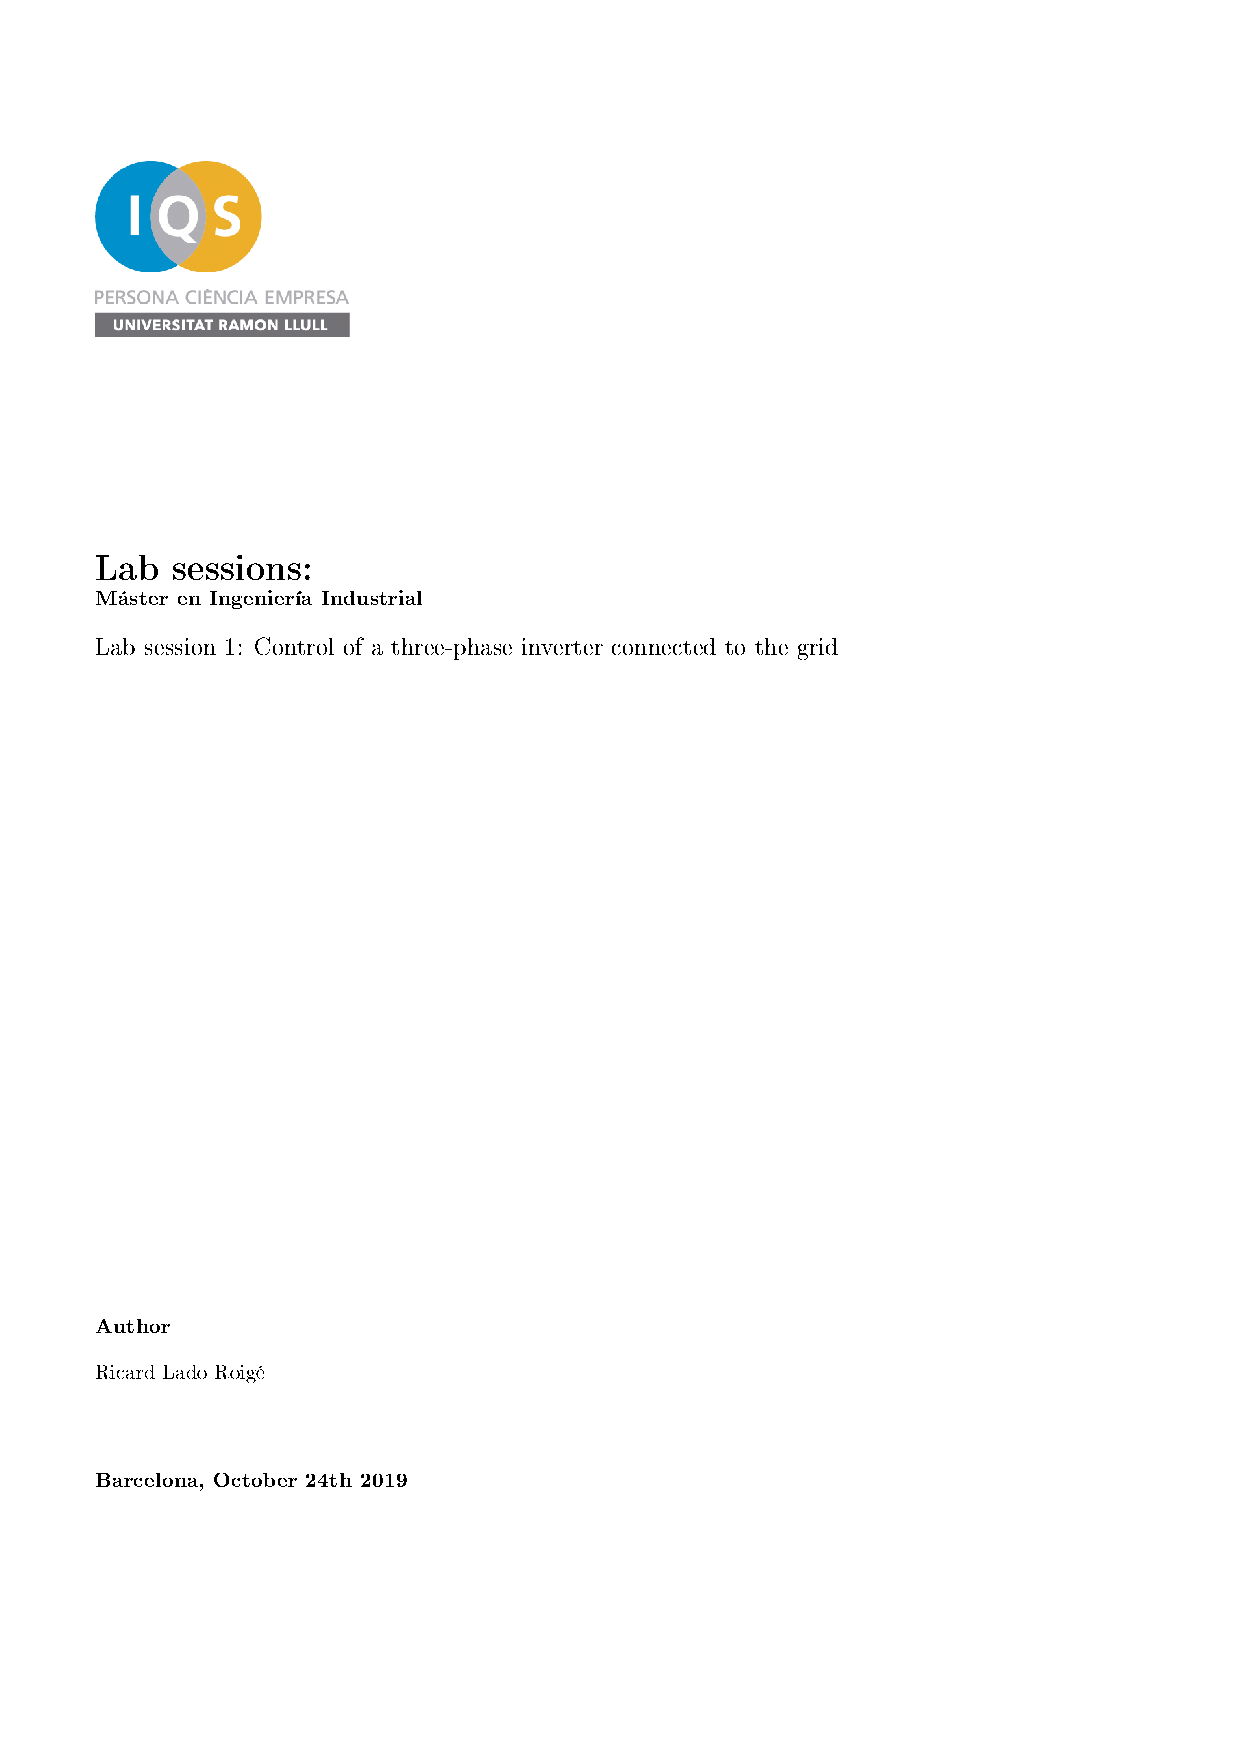
\includepdf[pages=-]{Chapters/S1_Report.pdf}

	\chapter{Report of lab session 2}
	\label{S2Report}
	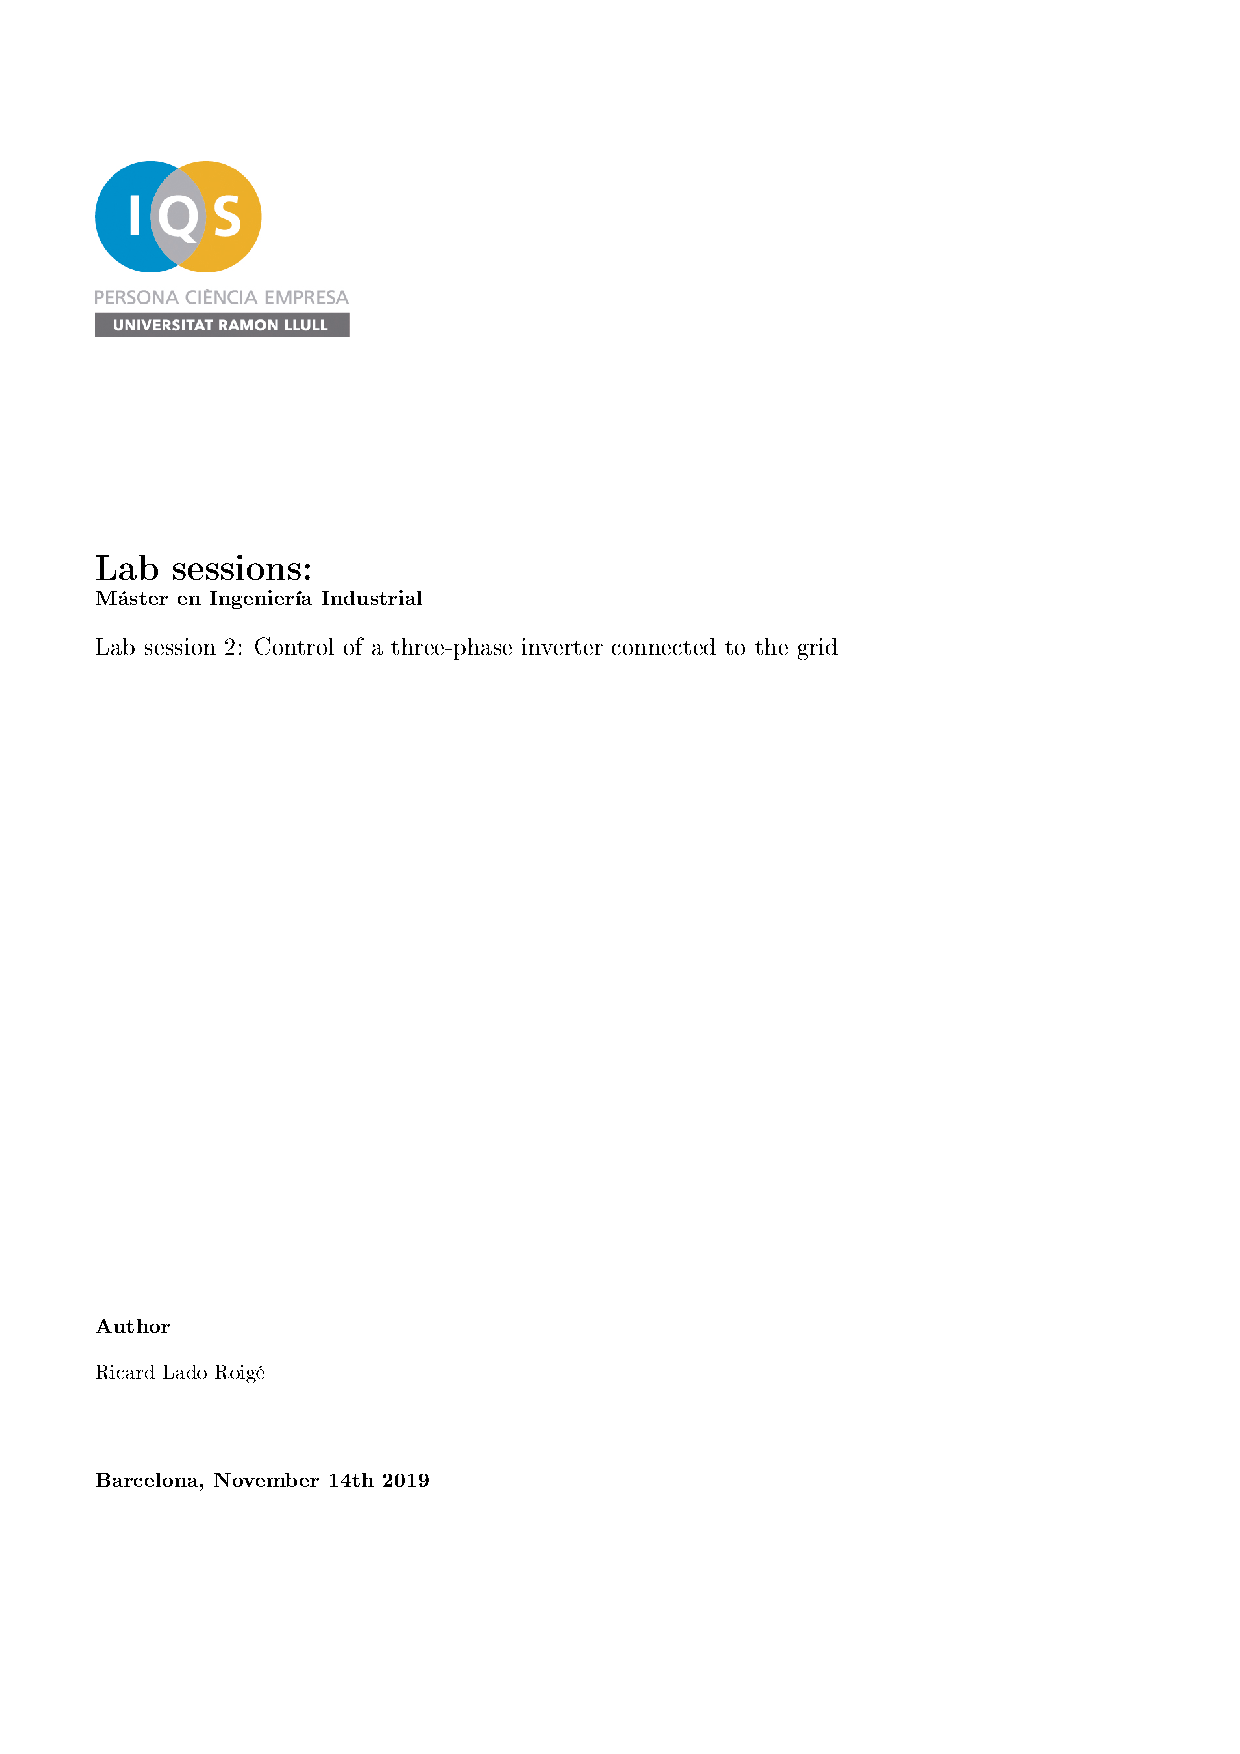
\includepdf[pages=-]{Chapters/S2_Report.pdf}

	\chapter{Report of lab session 3}
	\label{S3Report}
	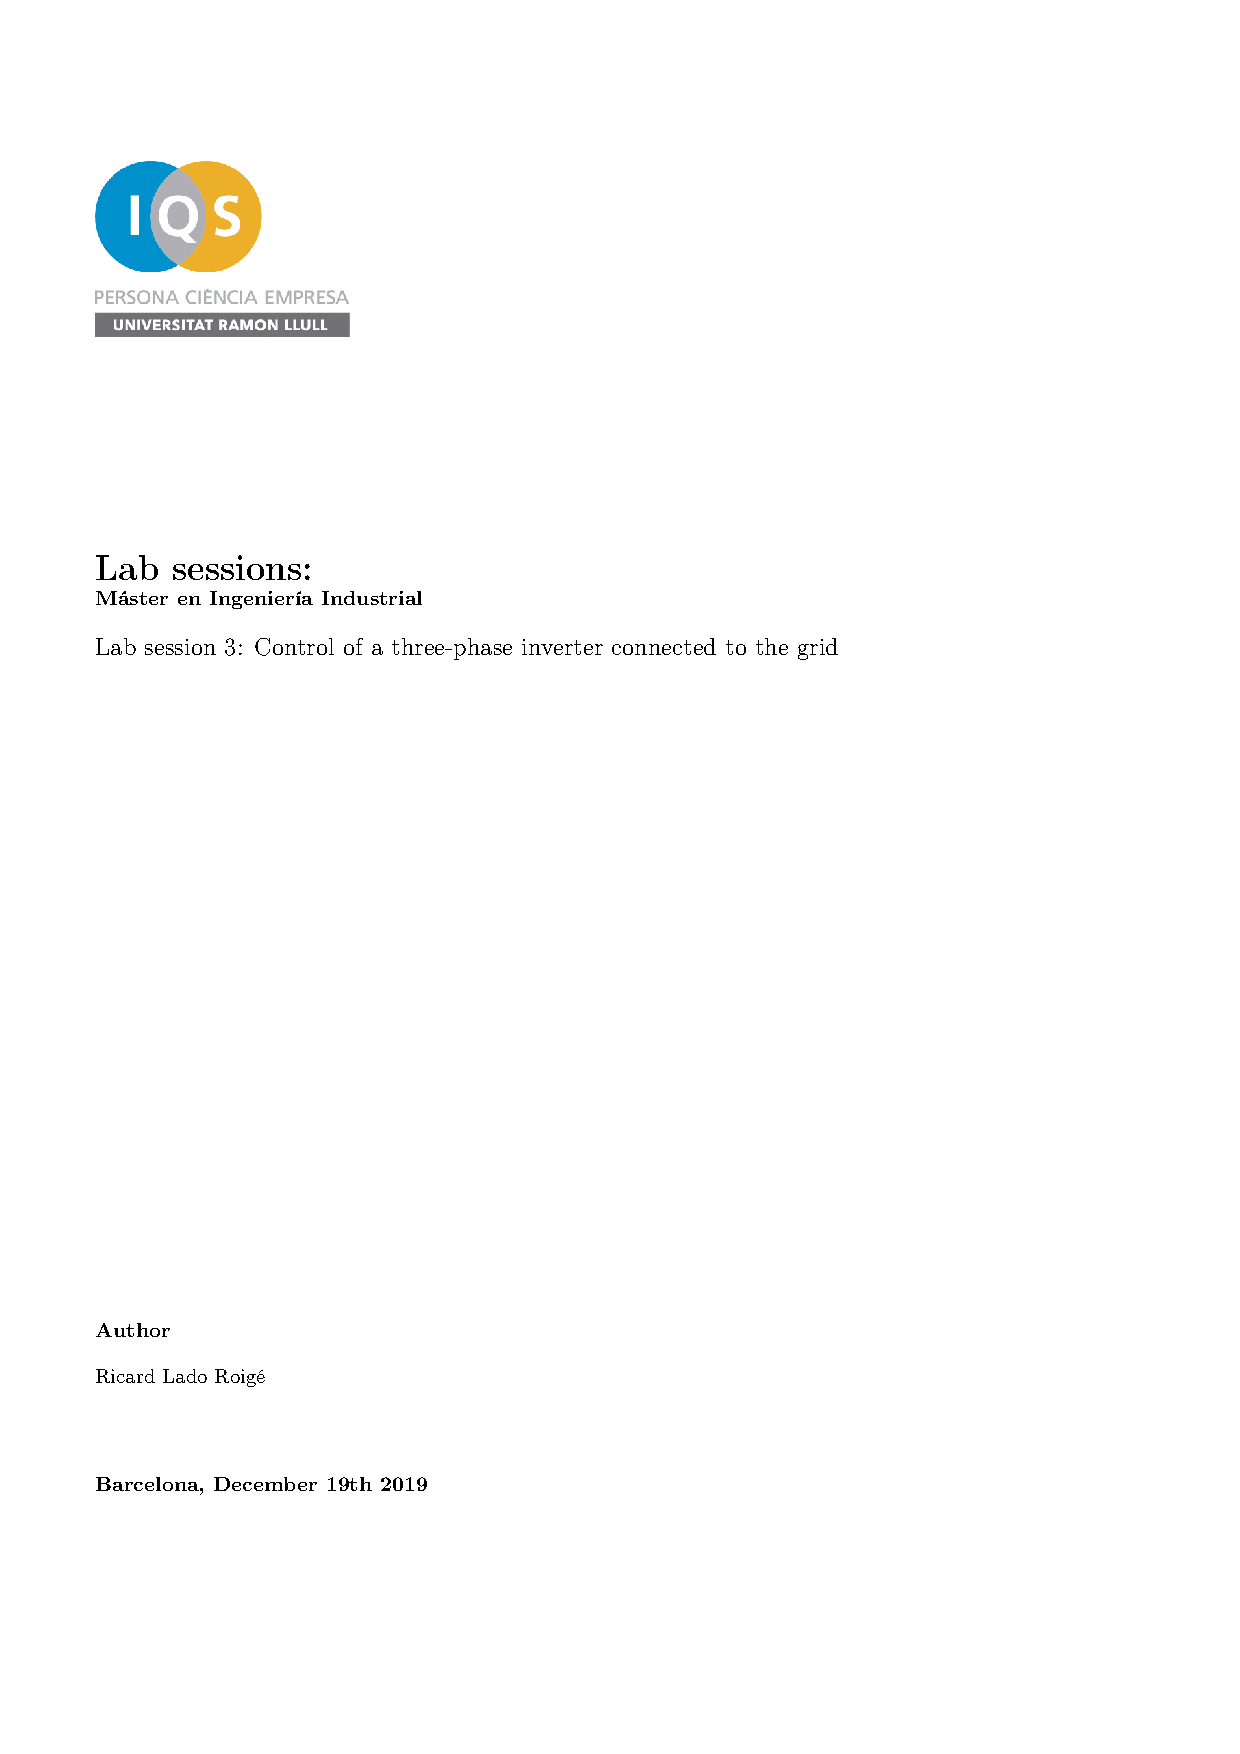
\includepdf[pages=-]{Chapters/S3_Report.pdf}

\end{document}
